\documentclass{beamer}
\usepackage[imecc]{collegeBeamer}
\usepackage[brazil]{babel}
\usepackage[utf8]{inputenc}
\usepackage{csquotes}
\usepackage{amsmath, amsfonts, amssymb, amsthm}
\usepackage{mathtools}
\usepackage{dsfont}
\usepackage{graphicx}
\usepackage{booktabs}
\usepackage{lmodern}
\usepackage{multirow}
\usepackage{multicol}
\usepackage{ragged2e}
\usepackage[alf]{abntex2cite}
\usepackage{tikz}
\makeatletter
\patchcmd{\beamer@checkframetitle}{\framesubtitle{\thesection \, \secname}}{}{}{}
\makeatother
\usetikzlibrary{arrows, positioning, shapes.geometric}

\setbeamertemplate{footline}{%
  \begin{beamercolorbox}[wd=\textwidth, ht=5mm, dp=3mm, rightskip=1cm]{footline}
    \usebeamerfont{footline}\hfill\insertframenumber
  \end{beamercolorbox}%
}

\title{Inferência causal em dados funcionais\\via transformadas de ondaletas}
\subtitle{do pré-processamento à estimação em tempo real}
\author{Moisés Augusto Farias da Silva \\ {\small Orientador: Prof.\ Dr.\ Alex Rodrigo dos Santos Sousa}}
\date{Instituto de Matemática, Estatística e Computação Científica \\ Universidade Estadual de Campinas \\ Maio de 2026}

\begin{document}

\maketitle

\begin{frame}{Sumário}
    \tableofcontents[hideallsubsections]
\end{frame}

% ===================================================
\section{Introdução}
% ===================================================

\begin{frame}{Contexto}
\begin{itemize}
    \item Inferência tradicional, inferência causal e análise de dados funcionais (FDA).
    \item Intersecção entre inferência causal e FDA em fase embrionária.
    \item \(N\) unidades \(i = 1, \ldots, N\), cada uma com tratamento \(A_i \in \{0,1\}\), covariáveis \(\mathbf{X}_i \in \mathbb{R}^P\) e trajetória funcional \(Y_i(t)\), \(t \in \mathcal{T}\), observada em \(T\) pontos discretos com ruído.
    \item Estimando de interesse: FATE (Functional Average Treatment Effect),
    \[
        \theta(t) = \mathbb{E}[Y^{(1)}(t) - Y^{(0)}(t)].
    \]
\end{itemize}
\end{frame}

\begin{frame}{Motivação}
\begin{itemize}
    \item A literatura usa métodos globais de suavização (e.g., B-\textit{splines}) para recuperar \(Y_i(t)\):
    \begin{itemize}
        \item Não robustos a perturbações locais.
        \item Exigem acesso à trajetória completa para estimativas estáveis.
        \item Em cenários mais complexos, podem violar a ``seta do tempo'' ao usarem dados futuros no pré-processamento.
    \end{itemize}
\end{itemize}
\end{frame}

\begin{frame}{Objetivos}
\begin{itemize}
    \item Propor ondaletas como pré-processamento para estimação do FATE.
    \begin{itemize}
        \item Utilização de \textit{lifting scheme} por sua extensibilidade, eficiência computacional e capacidade de processamento incremental.
        \item Implementação via pacote autoral \texttt{rLifting}, disponível no CRAN.
    \end{itemize}
    \medskip
    \item Propor estimador sequencial do FATE: estimativas são atualizadas à medida que novos dados chegam, respeitando a seta do tempo e possibilitando atualizações em tempo (quase) real.
\end{itemize}
\end{frame}

% ===================================================
\section{Referencial Teórico}
% ===================================================

\subsection{Inferência Causal Funcional}

\begin{frame}{Suposições de Identificabilidade}
\vspace{0.4cm}
Seja \(a \in \{0,1\}\) e \(Y_i^{(a)}(t)\) o resultado potencial de \(i\) sob \(a\).
\begin{enumerate}
    \item Ignorabilidade média: \(\mathbb{E}[Y^{(a)}(t) \mid A, \mathbf{X}] = \mathbb{E}[Y^{(a)}(t) \mid \mathbf{X}]\).
    \item Positividade: \(0 < \pi_a(\mathbf{X}_i) < 1\) q.c., \(\forall a \in \mathcal{A}\), em que \(\pi_a(\mathbf{X}_i) = \mathbb{P}(A_i = a \mid \mathbf{X}_i)\).
    \item Consistência: \(A_i = a \Rightarrow Y_i(t) = Y_i^{(a)}(t)\).
    \item Ausência de interferência (SUTVA).
\end{enumerate}
\medskip
Sob as quatro suposições:
\begin{align*}
    \theta(t)
    &= \mathbb{E}[Y^{(1)}(t) - Y^{(0)}(t)] = \mathbb{E}\!\left[Y^{(1)}(t)\right] - \mathbb{E}\!\left[Y^{(0)}(t)\right] \\
    &= \mathbb{E}\!\Big[\mathbb{E}[Y(t)\mid A{=}1,\mathbf{X}] - \mathbb{E}[Y(t)\mid A{=}0,\mathbf{X}]\Big].
\end{align*}
\end{frame}

\begin{frame}{\citeonline{ecker_causal_2024} — Modelo e Estimador}
\begin{itemize}
    \item Modelo linear funcional com erros MGP (independência entre indivíduos; correlação temporal via \(\sigma_a(s,t) = \mathrm{Cov}(\epsilon_i^{(a)}(s),\epsilon_i^{(a)}(t))\)):
    \[
        Y_i^{(a)}(t) = \mathbf{X}_i^\top \boldsymbol{\beta}^{(a)}(t) + \epsilon_i^{(a)}(t).
    \]
    \item Efeito heterogêneo: \(Y_i^{(1)}(t) - Y_i^{(0)}(t) = \mathbf{X}_i^\top\!\left(\boldsymbol{\beta}^{(1)}(t) - \boldsymbol{\beta}^{(0)}(t)\right).\)
    \item B-\textit{splines} \(\to\) MQO por grupo \(a\) \(\to\) estimador:
    \[
        \hat{\theta}(t) = \bar{\mathbf{X}}^\top\!\left(\hat{\boldsymbol{\beta}}^{(1)}(t) - \hat{\boldsymbol{\beta}}^{(0)}(t)\right).
    \]
\end{itemize}
\end{frame}

\begin{frame}{\citeonline{ecker_causal_2024} — Inferência}
\begin{itemize}
    \item A estrutura MGP induz covariância para \(\hat{\theta}(t)\):
    \[
        C_\theta(s,t) = \sigma_1(s,t)\,\bar{\mathbf{X}}^\top(\mathbf{X}_1^\top\mathbf{X}_1)^{-1}\bar{\mathbf{X}}
                      + \sigma_0(s,t)\,\bar{\mathbf{X}}^\top(\mathbf{X}_0^\top\mathbf{X}_0)^{-1}\bar{\mathbf{X}}.
    \]
    \item MQO linear + MGP \(\Rightarrow\) \(\hat{\theta}(t)\) gaussiano \(\Rightarrow\) bandas simultâneas de nível \(1{-}\alpha\):
    \[
        \mathbb{P}\!\left(\theta(t) \in \hat{\theta}(t) \pm u_\alpha(t)\sqrt{C_\theta(t,t)},\; \forall\, t\right) \geq 1 - \alpha.
    \]
    \item \(u_\alpha(t)\) é estimado na prática com ferramentas de inferência sobre processos gaussianos (e.g., pacote \texttt{ffscb}).
\end{itemize}
\end{frame}

\begin{frame}{Limitações de Primeira Ordem}
\begin{itemize}
    \item Estimador pontual: B-\textit{splines} não são robustos a perturbações locais; estimação sequencial inviável sem re-executar todo o procedimento.
    \medskip
    \item Bandas: operações não lineares no pré-processamento (limiarização, validação cruzada dos \textit{splines}) quebram a gaussianidade de \(\hat{\theta}(t)\) e invalidam as bandas analíticas.
\end{itemize}
\end{frame}

\begin{frame}{Outros trabalhos em Inf. Causal Funcional}
\begin{itemize}
    \item \citeonline{testa_doubly-robust_2025} — duplamente robusto; suaviza o pseudo-desfecho após a estimação. Pode carregar ruído indesejável para a etapa de estimação.
    \item \citeonline{sparkes_functional_2024} — substituem a ignorabilidade por restrição distribucional: o desfecho potencial condicional \(Y^{(a)}(t)\mid\mathbf{X}\) deve pertencer à classe \(\mathcal{U}\) (\(\mathbb{E}[Z] = \mathrm{Av}(Z)\); satisfeita por distribuições simétricas).
    \item \citeonline{wong_kernel-based_2018} — covariáveis funcionais, ATE escalar; balanceamento via \textit{kernel}.
    \item \citeonline{colantuoni_statistical_2018} — desfechos funcionais com censura informativa. Estrutura de dados mais especializada, fora do escopo Neyman--Rubin padrão.
    \item \citeonline{kikuchi_dynamic_2025} — efeitos de trajetórias de exposição no espaço-tempo. Problema estruturalmente diferente desde a concepção.
\end{itemize}
\end{frame}

\subsection{Ondaletas}

\begin{frame}{Sinal e Ondaletas}
\begin{itemize}
    \item Assumiremos \(f_i(t) \in L^{2}(\mathbb{R})\), \(t \in \mathcal{T}\), \(\forall i\).
    \item Sinal observado: \(Y_i[k] = f_i(t_k) + \eta_{i,k}\), \(k=0,\ldots,T{-}1\), \(T = 2^J\) (\(J\) = número de níveis de resolução). No contexto causal, \(f_i(t_k) \equiv Y_i(t_k)\) é a trajetória latente a recuperar.
    \item Ondaletas: funções com média nula e energia finita; localizadas no tempo e na frequência.
    \begin{itemize}
        \item Alta resolução temporal para eventos rápidos (picos, descontinuidades).
        \item Energia do sinal concentra-se em poucos coeficientes grandes; ruído distribui-se uniformemente.
        \item Em \textit{splines}, perturbações locais propagam-se pela base inteira.
    \end{itemize}
\end{itemize}
\end{frame}

\begin{frame}{Hipóteses sobre o Ruído}
\begin{itemize}
    \item Supomos \(\eta_{i,k} \overset{\mathrm{iid}}{\sim} N(0, \sigma^2)\).
    \begin{itemize}
        \item Normalidade razoável para erros de medição; limiarização é relativamente robusta a desvios leves.
        \item iid é a hipótese mais sensível: autocorrelação em dados temporais viola independência e viesa a estimativa de \(\sigma\) via MAD.
        \item A DWT atua como decorrelacionador em muitos regimes, atenuando esse impacto na prática.
    \end{itemize}
\end{itemize}
\end{frame}

\begin{frame}{DWT e \textit{Lifting Scheme}}
\begin{itemize}
    \item DWT decompõe \(Y_i[k]\) em coeficientes de aproximação \(s_{i,j}[\kappa]\) e detalhe \(d_{i,j}[\kappa]\), iterando \(j = J, \ldots, 1\).
    \item \textit{Lifting scheme}: implementação modular da DWT, sem banco de filtros, sem memória auxiliar.
    \begin{enumerate}
        \item Separação: pares \(s_{i,j,\text{par}}\) e ímpares \(s_{i,j,\text{ímpar}}\).
        \item Predição (\(\mathcal{P}\)): \(d_{i,j}[\kappa] = s_{i,j,\text{ímpar}}[\kappa] - \mathcal{P}(s_{i,j,\text{par}}[\kappa])\).
        \item Atualização (\(\mathcal{U}\)): \(s_{i,j}[\kappa] = s_{i,j,\text{par}}[\kappa] + \mathcal{U}(d_{i,j}[\kappa])\).
        \item Normalização.
    \end{enumerate}
    \item ILWT: desfaz cada passo em ordem reversa. \(\mathcal{P}\) e \(\mathcal{U}\) customizáveis.
\end{itemize}
\end{frame}

\begin{frame}{Limiarização de Coeficientes}
\begin{itemize}
    \item \(d_{i,j}[\kappa] = D_{i,j}[\kappa] + \rho_{i,j}[\kappa]\); objetivo: suprimir \(\rho\) preservando \(D\) via limiar \(\lambda > 0\).
    \medskip
    \item Limiarização dura: \(\delta^H(d) = d \cdot \mathbb{I}(|d| > \lambda)\).
    \item Limiarização suave: \(\delta^S(d) = \mathrm{sgn}(d)(|d| - \lambda)_+\).
    \item Limiar universal \cite{donoho_ideal_1994}: \(\lambda = \hat{\sigma}\sqrt{2\log T}\), \(\hat{\sigma} = \mathrm{MAD}(|d_{i,J-1}[\kappa]|)/0{,}6745\).
\end{itemize}
\end{frame}

\begin{frame}{Limiarização Semisuave e Limiar Adaptativo}
\begin{itemize}
    \item Semisuave \cite{liu_improved_2014}: compromisso entre dura e suave. Usada neste trabalho.
    \[
        \hat{d}_{i,j}[\kappa] = \begin{cases}
            \mathrm{sgn}(d_{i,j}[\kappa])\sqrt{d_{i,j}[\kappa]^2 - \lambda^2}, & |d_{i,j}[\kappa]| > \lambda, \\
            0, & |d_{i,j}[\kappa]| \leqslant \lambda.
        \end{cases}
    \]
    \item Limiar adaptativo por nível \(j\) (hiper-parâmetros \(\alpha \in (0,1)\), \(\beta > 1\)):
    \[
        \lambda_j = \begin{cases}
            \beta \cdot \dfrac{\mathrm{MAD}(|d_{i,J-1}[\kappa]|)}{0{,}6745}\sqrt{2\log T_{J-1}}, & j = J-1, \\[4pt]
            \dfrac{j+1}{j+1+\alpha}\,\lambda_{j+1}, & j < J-1.
        \end{cases}
    \]
\end{itemize}
\end{frame}

\begin{frame}{Pré-processamento Sequencial}
\begin{itemize}
    \item Processamos \(Y_i[k]\) usando apenas \(Y_i[0], \ldots, Y_i[k]\).
    \item Janela móvel \(W = 2^L\) (\(L \in \mathbb{N}\) escolhido pelo analista; dentro da janela, \(J = L\)):
    \begin{itemize}
        \item \(k < W-1\): retorna \(Y_i[k]\) bruto (janela incompleta).
        \item \(k \geq W-1\): aplica DWT, limiarização e ILWT; retorna \(\hat{Y}_i[k]\).
    \end{itemize}
    \item Cada \(\hat{Y}_i[k]\) depende exclusivamente de dados passados — causalidade operacional por construção.
    \item Extensão de bordas: simétrica em ambos os modos; no modo \textit{online} recomendamos filtros curtos (Haar, Daubechies-2) para minimizar artefatos de borda direita.
\end{itemize}
\end{frame}

% ===================================================
\section{Metodologia}
% ===================================================

\begin{frame}{\texttt{rLifting}}
\begin{itemize}
    \item Pacote R/C++ para DWT causal com processamento sequencial; disponível no CRAN.
    \item Nenhum pacote existente combinava limiarização automática e causalidade operacional; \texttt{adlift} e \texttt{nlt} levam segundos por sinal — inviáveis para simulações de Monte Carlo ou tempo real.
    \item Implementa LWT, ILWT, limiarização (dura, suave, semisuave) e limiar adaptativo recursivo.
    \item 6 famílias pré-configuradas; extensível via \texttt{lift\_step} + \texttt{custom\_wavelet}; \texttt{diagnose\_wavelet} valida consistência.
    \item Interfaces: \texttt{denoise\_signal\_offline}, \texttt{denoise\_signal\_causal}, \texttt{new\_wavelet\_stream}.
\end{itemize}
\end{frame}

\begin{frame}{\texttt{rLifting} — Desempenho}
\vspace{0.4cm}
Sinal \textit{Doppler} \cite{donoho_ideal_1994}: frequência variável, \(T{=}1024\), \(\sigma{=}0.3\), modo \textit{offline}, 50 réplicas.

\medskip
\begin{columns}[c]
\column{0.44\textwidth}
\begin{table}
\centering
{\small
\begin{tabular}{lc}
\toprule
\textbf{Pacote} & \textbf{Mediana (ms)} \\
\midrule
\texttt{rLifting}   & \textbf{0.046} \\
\texttt{wavethresh} & 1.240 \\
\texttt{nlt}        & 2507.970 \\
\texttt{adlift}     & 2582.440 \\
\bottomrule
\end{tabular}
}
\caption{\scriptsize Tempo mediano de execução (DWT + limiarização + ILWT), 50 réplicas.}
\end{table}

\column{0.52\textwidth}
\begin{figure}
\centering
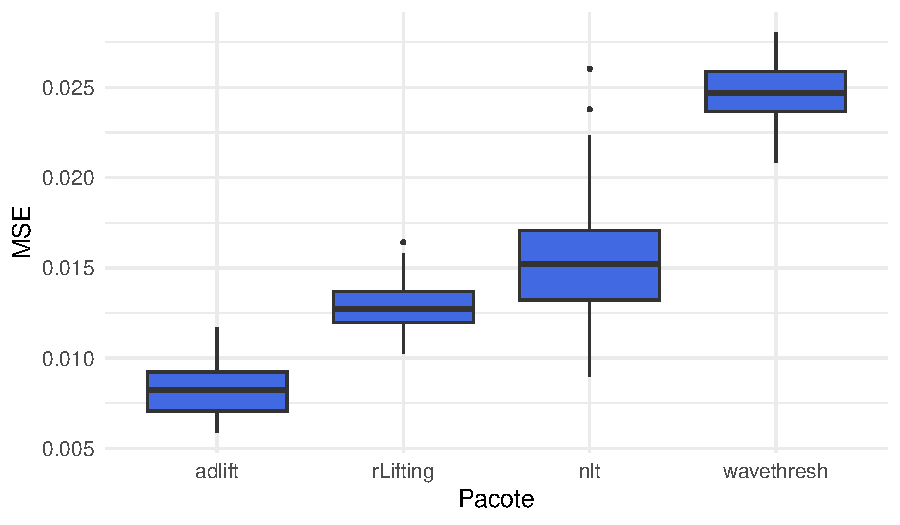
\includegraphics[width=0.86\textwidth]{../figuras/benchmark_mse.pdf}
\caption{\scriptsize Distribuição do MSE de reconstrução, 50 réplicas. Menores valores indicam maior precisão.}
\end{figure}
\end{columns}
\end{frame}

\begin{frame}{Estimadores do FATE}
\begin{itemize}
    \item Pré-processamento via ondaletas (análogo a \citeonline{ecker_causal_2024}, mas com DWT via \textit{lifting}):
    \begin{itemize}
        \item \textit{Offline}: sinal completo \(\{Y_i[0],\ldots,Y_i[T{-}1]\}\); \(J = \log_2(T)\) níveis; extensão simétrica.
        \item \textit{Online}: janela móvel \(W = 2^L\) (\(L \in \mathbb{N}\), número de níveis); apenas \(Y_i[0], \ldots, Y_i[k]\) disponíveis a cada \(k\).
    \end{itemize}
    \item Limiarização semisuave com limiar adaptativo (\(\alpha{=}0.3\), \(\beta{=}1.2\)) nos dois modos.
\end{itemize}
\end{frame}

\begin{frame}{Estimadores do FATE II}
\begin{itemize}
    \item Estimação pontual (idêntica nos dois modos): MQO por grupo \(a\) sobre \(\hat{Y}_i(t)\):
    \[
        \hat{\theta}(t) = \bar{\mathbf{X}}^\top\!\left(\hat{\boldsymbol{\beta}}^{(1)}(t) - \hat{\boldsymbol{\beta}}^{(0)}(t)\right).
    \]
    \item Modo \textit{online}: matriz de projeção \(\mathbf{P}^{(a)}_\lambda = (\mathbf{X}_a^\top\mathbf{X}_a + \lambda_\text{Ridge}\mathbf{I})^{-1}\mathbf{X}_a^\top\) calculada uma única vez. A cada \(k\):
    \[
        \hat{\boldsymbol{\beta}}^{(a)}(t_k) = \mathbf{P}^{(a)}_\lambda\,\mathbf{y}^{(a)}[k]. \quad \text{(microssegundos por ponto)}
    \]
\end{itemize}
\end{frame}

\begin{frame}{Estimadores do FATE III — Bandas de Confiança}
\begin{itemize}
    \item Limiarização viola gaussianidade de \(\hat{\theta}(t)\); bandas analíticas de \citeonline{ecker_causal_2024} inválidas.
    \item Solução: separar estimação pontual (com ondaletas) da incerteza (sem pré-processamento) \cite{chatterjee_bootstrapping_2011}.
    \item \textit{Bootstrap} para \(b = 1, \ldots, B\):
    \begin{enumerate}
        \item Reamostrar \(N\) unidades com reposição, preservando trajetória, \(A_i\) e \(\mathbf{X}_i\).
        \item Reestimar \(\hat{\theta}_b(t)\) por MQO sobre dados brutos.
        \item \(D_b = \max_{t \in \mathcal{T}} |\hat{\theta}_b(t) - \hat{\theta}(t)|\).
    \end{enumerate}
    \item Banda: \(\hat{\theta}(t) \pm q_{1-\alpha}\), em que \(q_{1-\alpha}\) é o percentil \(100(1{-}\alpha)\%\) de \(\{D_b\}\). Inviável em tempo real estrito.
\end{itemize}
\end{frame}

\begin{frame}{Propriedades Estatísticas do Estimador}
\begin{itemize}
    \item Viés: a limiarização introduz viés em amostras finitas. Assintoticamente, com \(N, T \to \infty\), o viés duplo desaparece.
    \item Consistência: o estimador decompõe-se em MQO (consistente com \(N\to\infty\)) e reconstrução por ondaletas (erro em \(L^2\) vai a zero com \(T\to\infty\)). Consistência global exige \(N, T \to \infty\) simultaneamente.
    \item Modo \textit{online}: causalidade operacional garantida por construção; consistência requer que \(W = W(T) \to \infty\) com \(T\).
    \item Bandas de confiança: cobertura nominal \(1-\alpha\) via \textit{bootstrap} (não paramétrico; não exige gaussianidade). Bandas de \citeonline{ecker_causal_2024} inválidas após limiarização.
\end{itemize}
\end{frame}

% ===================================================
\section{Estudos de Simulação}
% ===================================================

\begin{frame}{Configuração das Simulações}
\begin{itemize}
    \item PGD de \citeonline{ecker_causal_2024}: \(P{=}9\) covariáveis (Normal, Poisson, Binomial); atribuição logística; propensões em \([0.001, 0.999]\).
    \item 4 formas funcionais: Sigmoide, Bumps, Doppler, Escada.
    \item \(N \in \{200, 500, 2000\}\) \(\times\) \(T \in \{128, 256, 512\}\); \(R = 1000\) réplicas.
    \medskip
    \item Sim 1: ondaletas (\textit{offline} e \textit{online}) vs.\ \textit{splines} de \citeonline{ecker_causal_2024} (50 funções de base, GCV).
    \item Sim 2: estimador \textit{online} via \texttt{new\_wavelet\_stream}; foco em latência e fidelidade.
    \item Métricas: NRMSE, viés global, CobSim (nominal \(= 95\%\)).
\end{itemize}
\end{frame}

\begin{frame}{Simulação 1 — Resultados (I): Sigmoide e Doppler}
\begin{table}
\centering
{\scriptsize
\begin{tabular}{llccrrr}
\toprule
Cenário & Método & \(N\) & \(T\) & NRMSE & Viés & CobSim \\
\midrule
\multirow{6}{*}{Sigmoide}
 & Ond.\ (On)  & 200  & 128 & 0.574 & $0.055$ & 85.9\% \\
 & Ond.\ (Off) & 200  & 128 & 0.585 & $0.058$ & 86.6\% \\
 & Ecker       & 200  & 128 & 0.584 & $0.058$ & 100.0\% \\
\cmidrule{2-7}
 & Ond.\ (On)  & 2000 & 512 & 0.010 & $-$0.001 & 94.6\% \\
 & Ond.\ (Off) & 2000 & 512 & 0.010 &    0.000 & 95.0\% \\
 & Ecker       & 2000 & 512 & 0.010 &    0.000 & 100.0\% \\
\midrule
\multirow{6}{*}{Doppler}
 & Ond.\ (On)  & 200  & 128 & 0.161 & $0.027$ & 86.8\% \\
 & Ond.\ (Off) & 200  & 128 & 0.155 & $0.044$ & 86.8\% \\
 & Ecker       & 200  & 128 & 0.253 & $0.051$ & 40.1\% \\
\cmidrule{2-7}
 & Ond.\ (On)  & 2000 & 512 & 0.037 & $-$0.008 & \textbf{96.2\%} \\
 & Ond.\ (Off) & 2000 & 512 & \textbf{0.005} & $-$0.001 & \textbf{95.2\%} \\
 & Ecker       & 2000 & 512 & 0.130 &    0.000 & \textbf{0.0\%} \\
\bottomrule
\end{tabular}
}
\caption{\scriptsize Sigmoide: métodos equivalentes em precisão. Doppler: vantagem das ondaletas aumenta com \(N\) e \(T\); cobertura do Ecker colapsa a zero.}
\end{table}
\end{frame}

\begin{frame}{Simulação 1 — Resultados (II): Escada e Bumps}
\begin{table}
\centering
{\scriptsize
\begin{tabular}{llccrrr}
\toprule
Cenário & Método & \(N\) & \(T\) & NRMSE & Viés & CobSim \\
\midrule
\multirow{6}{*}{Escada}
 & Ond.\ (On)  & 200  & 128 & 0.046 & $0.084$ & 87.2\% \\
 & Ond.\ (Off) & 200  & 128 & 0.047 & $0.077$ & 88.0\% \\
 & Ecker       & 200  & 128 & 0.086 & $0.077$ & 40.8\% \\
\cmidrule{2-7}
 & Ond.\ (On)  & 2000 & 512 & \textbf{0.001} & $0.001$ & \textbf{95.5\%} \\
 & Ond.\ (Off) & 2000 & 512 & \textbf{0.001} & $0.000$ & \textbf{95.7\%} \\
 & Ecker       & 2000 & 512 & 0.039 & $0.000$ & \textbf{0.0\%} \\
\midrule
\multirow{6}{*}{Bumps}
 & Ond.\ (On)  & 200  & 128 & 0.021 & $0.131$ & 86.0\% \\
 & Ond.\ (Off) & 200  & 128 & 0.021 & $0.148$ & 86.1\% \\
 & Ecker       & 200  & 128 & 0.113 & $0.147$ & 40.8\% \\
\cmidrule{2-7}
 & Ond.\ (On)  & 2000 & 512 & \textbf{0.001} & $-$0.002 & \textbf{94.1\%} \\
 & Ond.\ (Off) & 2000 & 512 & \textbf{0.000} & $0.000$ & \textbf{96.0\%} \\
 & Ecker       & 2000 & 512 & 0.071 & $0.000$ & \textbf{0.0\%} \\
\bottomrule
\end{tabular}
}
\caption{\scriptsize Padrão consistente: ondaletas dominam Ecker em cenários de descontinuidade e picos abruptos.}
\end{table}
\end{frame}

\begin{frame}{Simulação 1 — Figuras (I)}
\begin{figure}
\centering
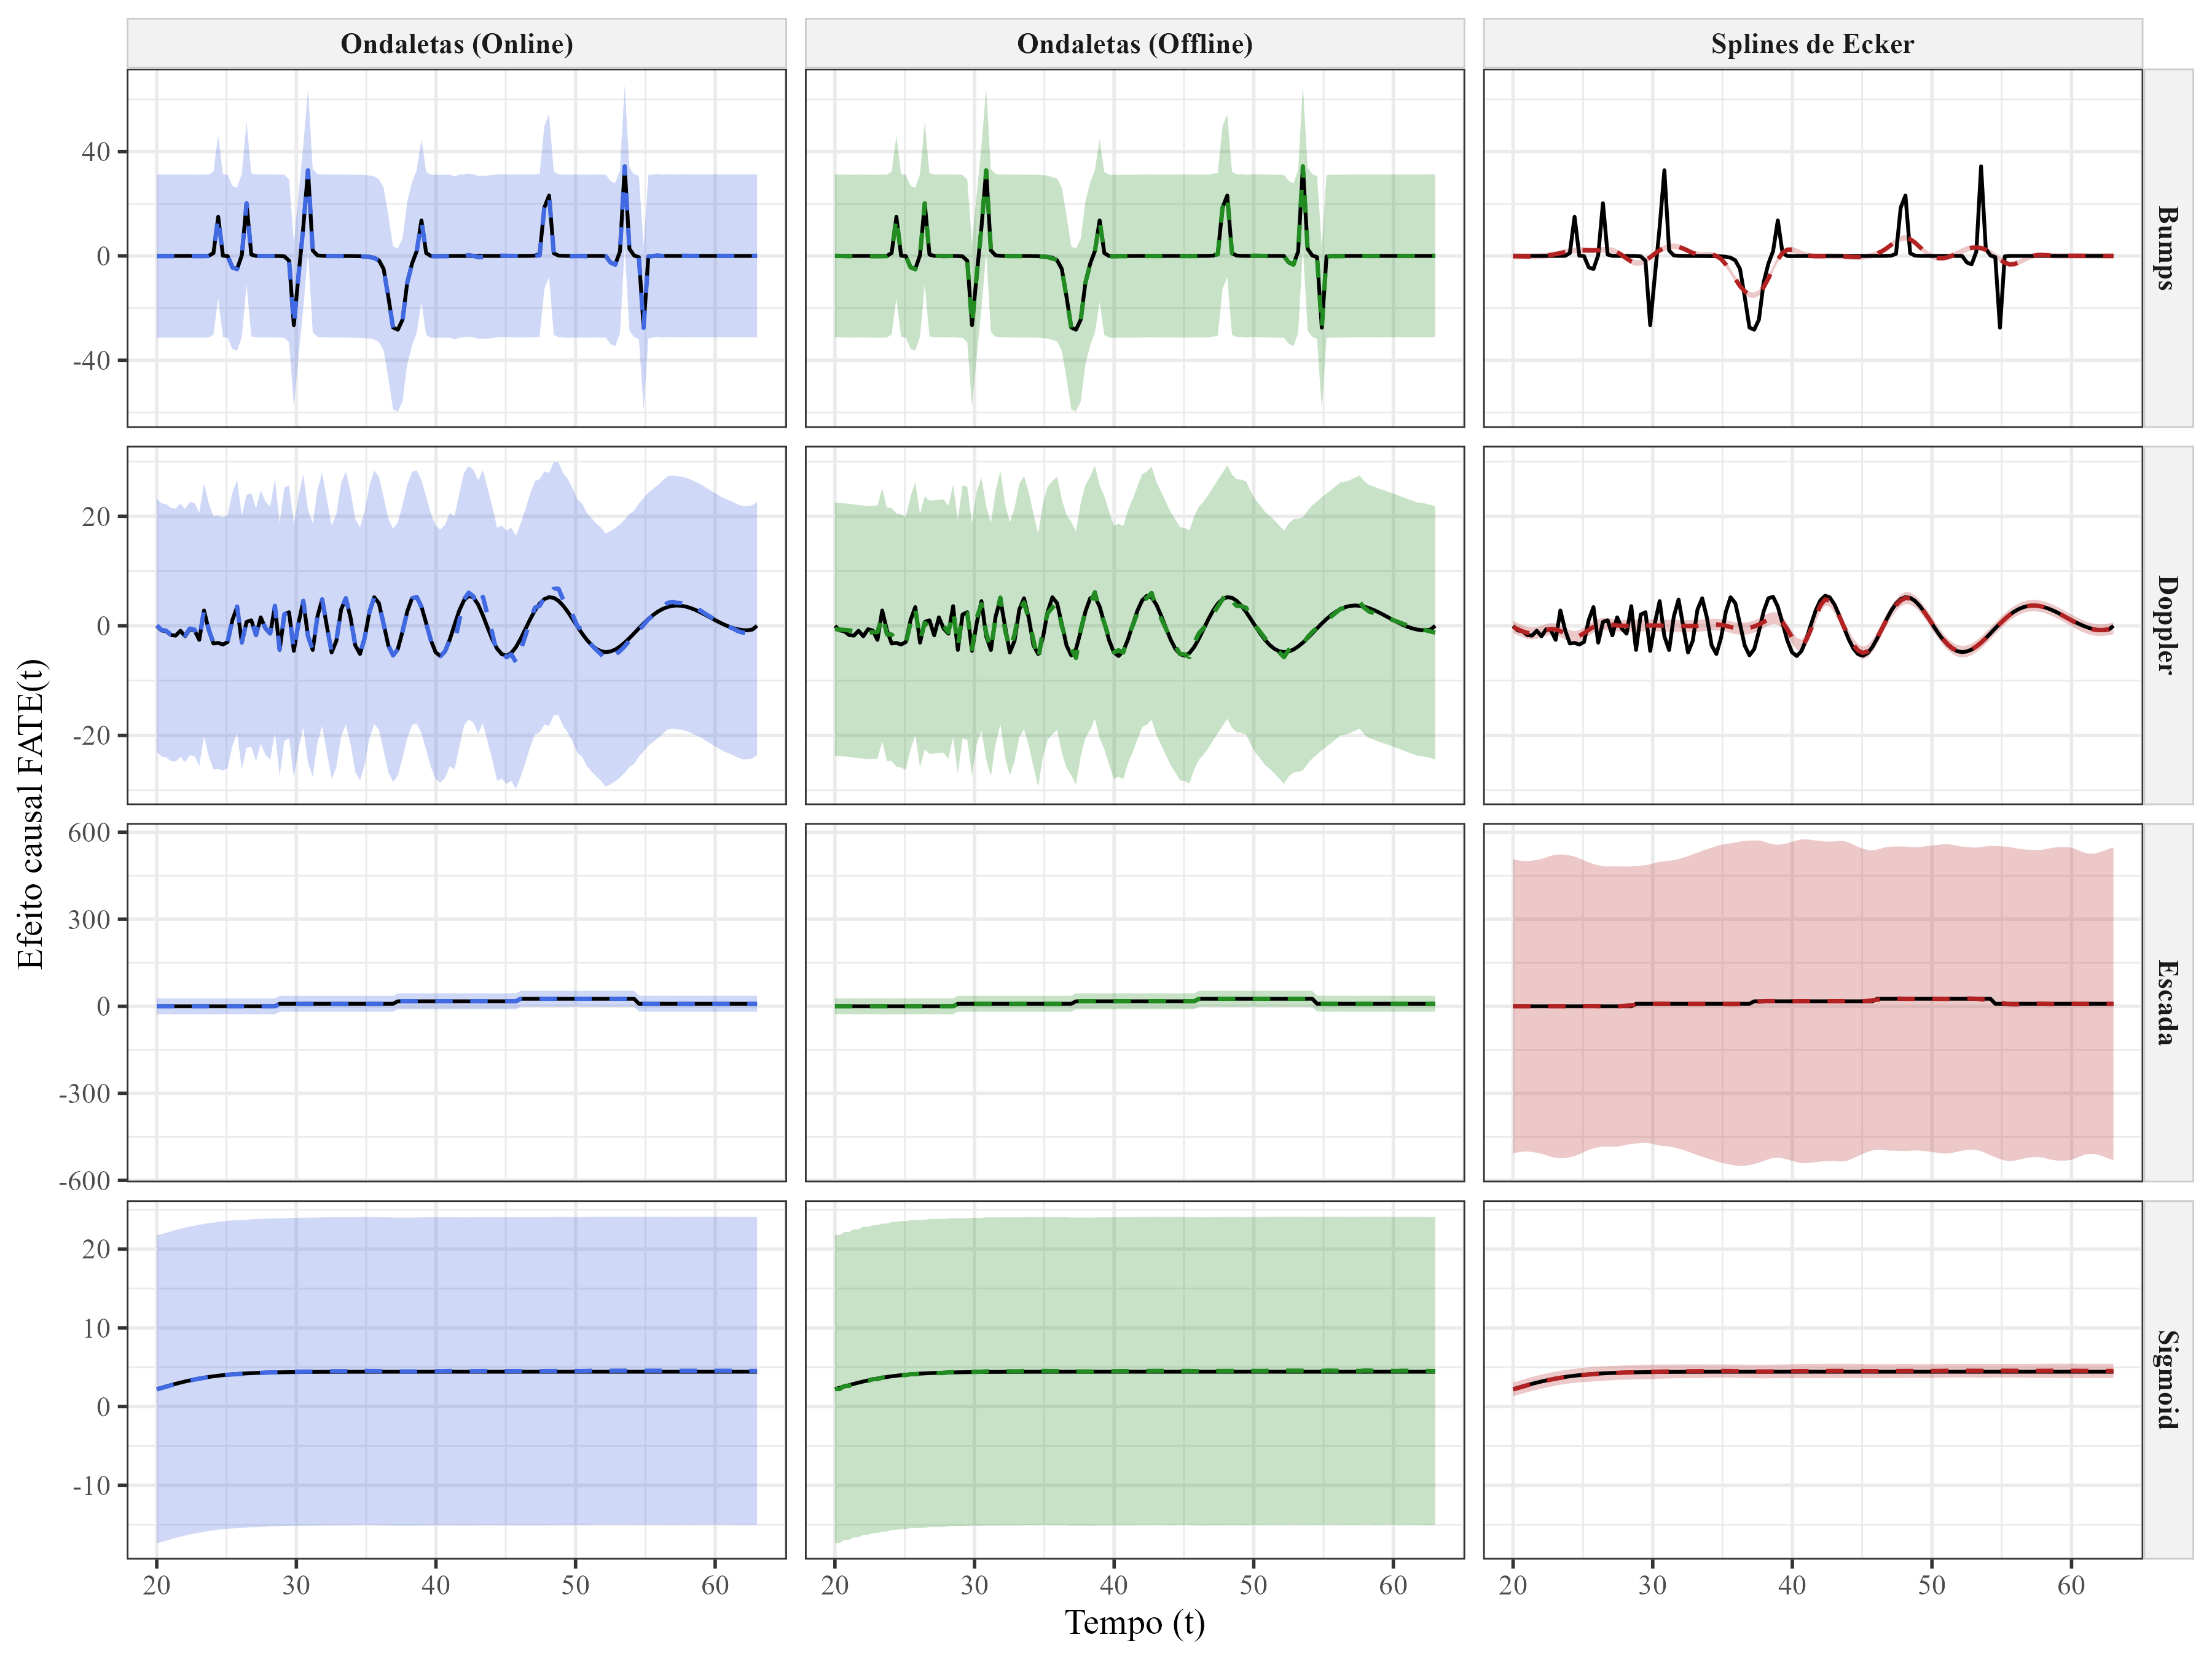
\includegraphics[height=0.95\textheight]{../figuras/sim1/texto_principal/exemplary_run_worst_case.png}
\caption{\scriptsize Pior caso (\(N=200\), \(T=128\)). Todos os métodos capturam a tendência central; bandas das ondaletas são mais realistas.}
\end{figure}
\end{frame}

\begin{frame}{Simulação 1 — Figuras (II)}
\begin{figure}
\centering
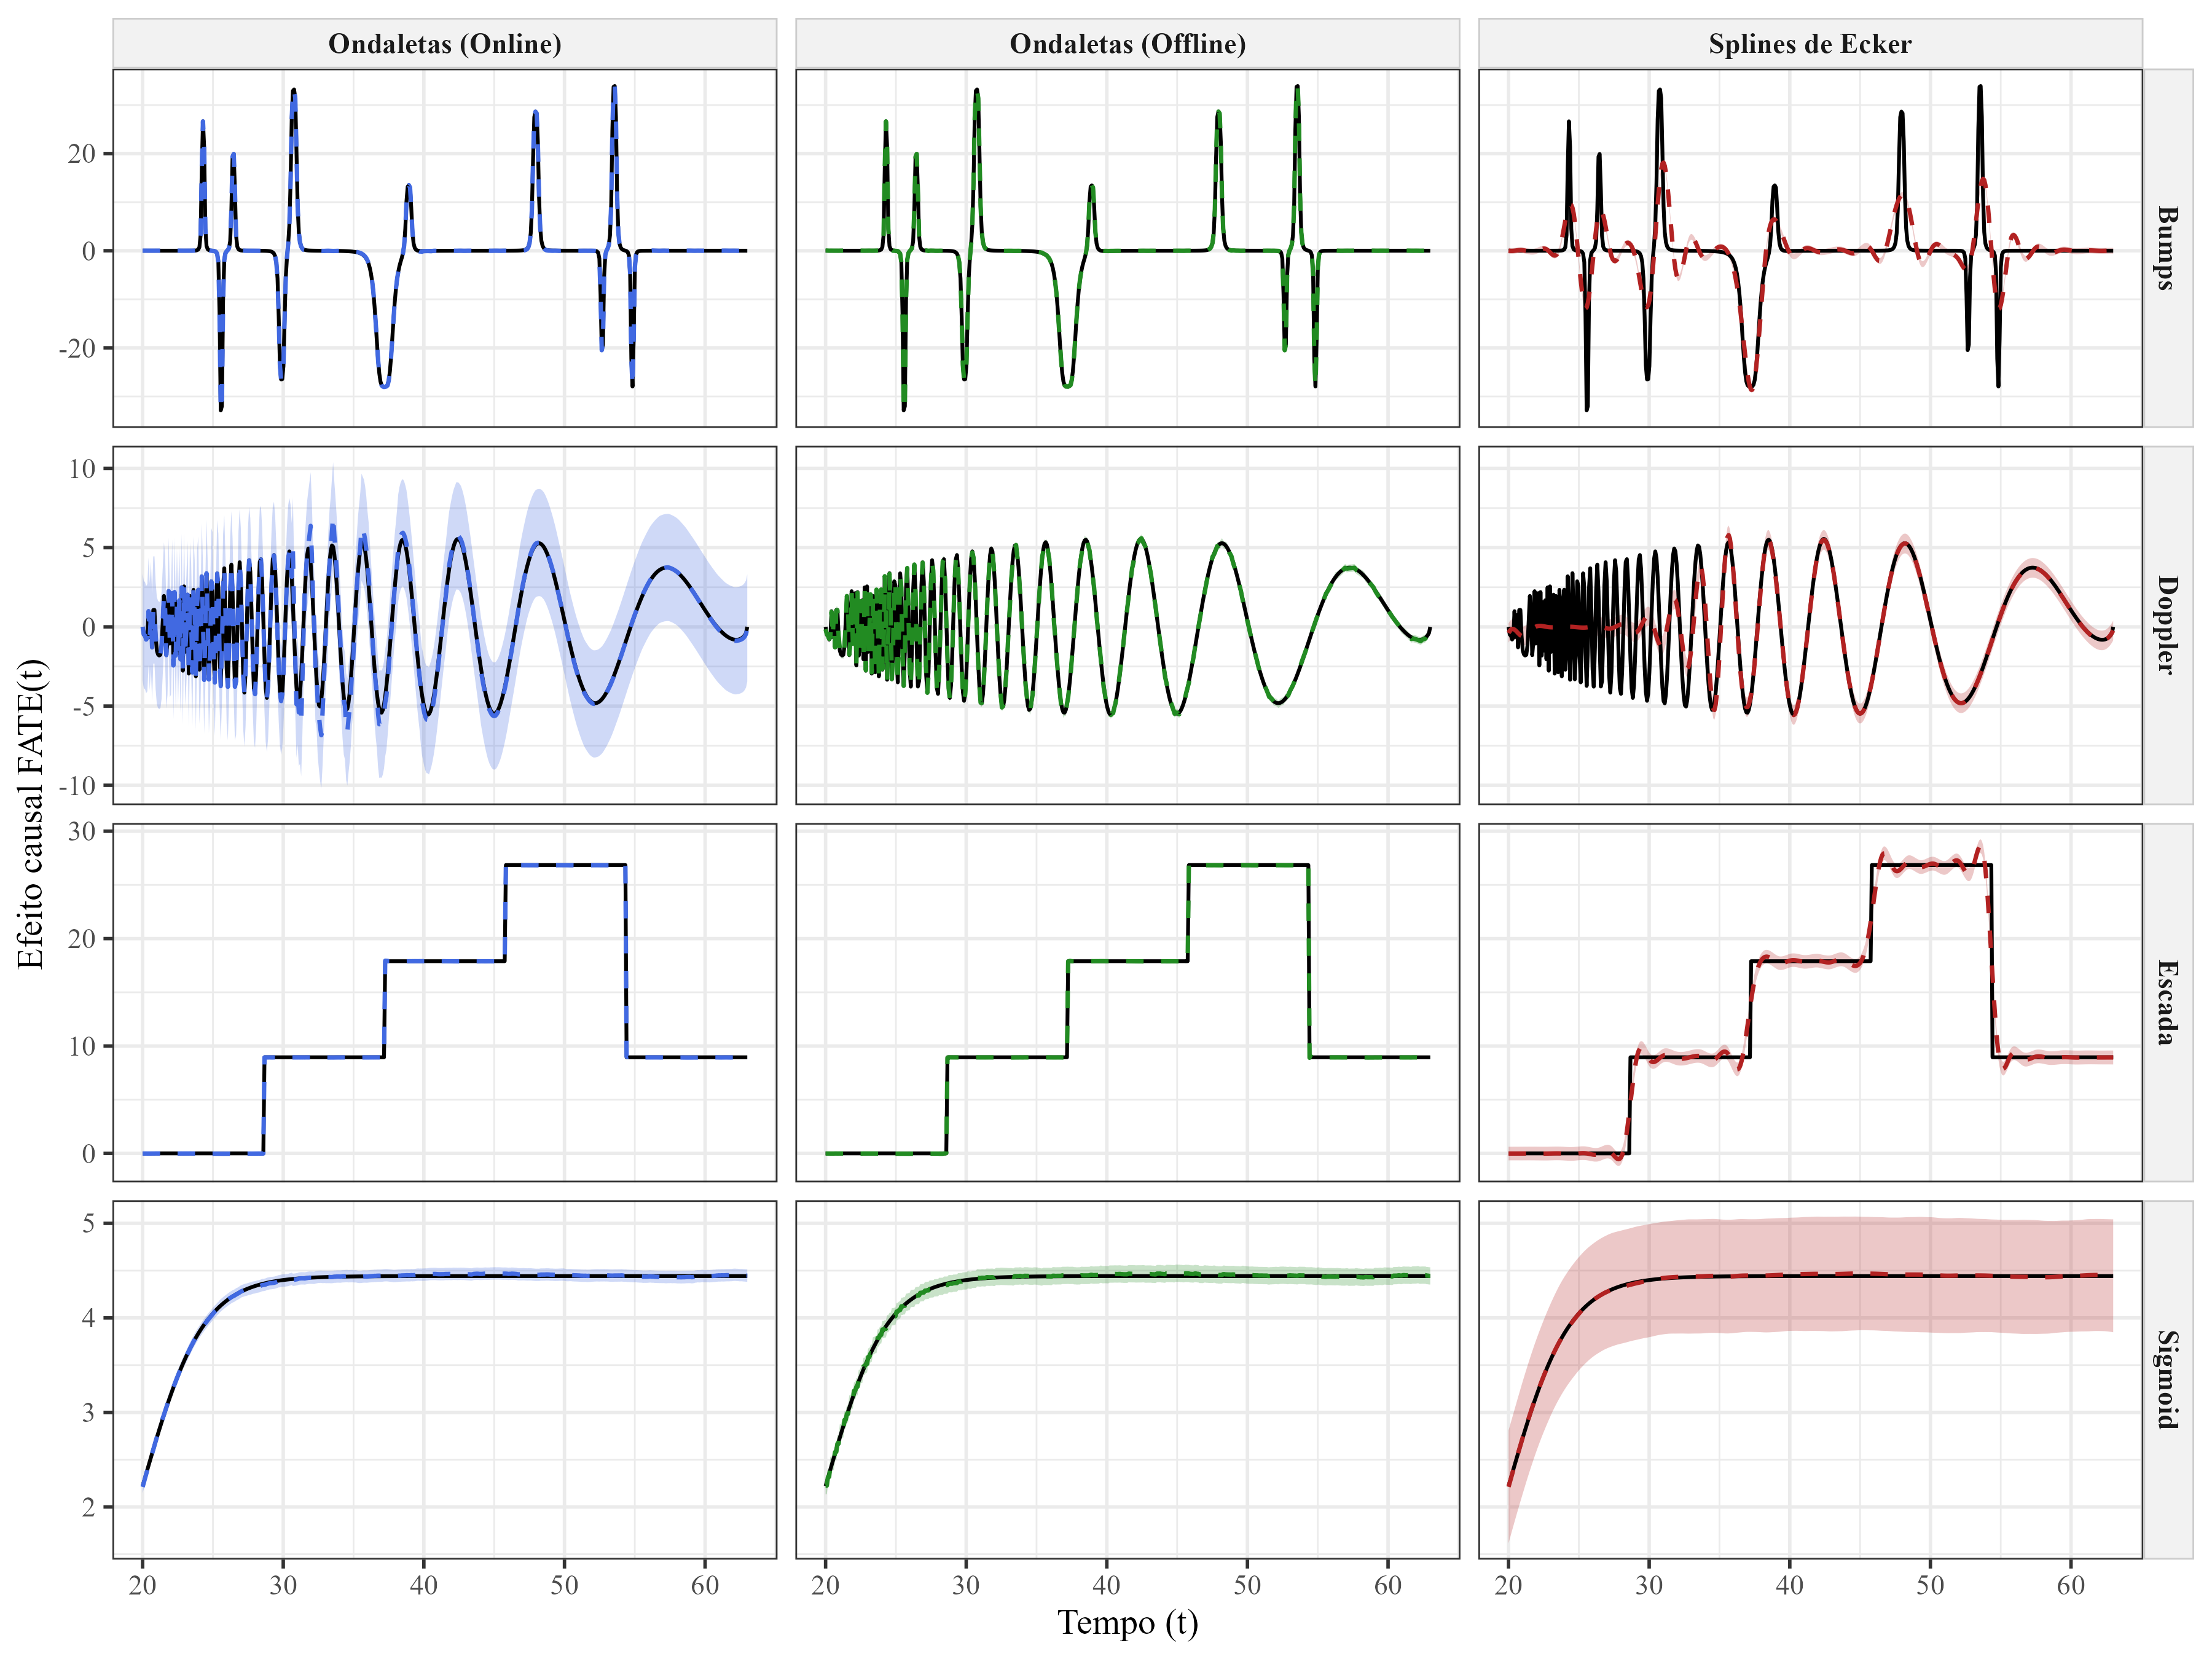
\includegraphics[height=0.95\textheight]{../figuras/sim1/texto_principal/exemplary_run_best_case.png}
\caption{\scriptsize Melhor caso (\(N=2000\), \(T=512\)). Ondaletas aderem à curva teórica; splines falham em Doppler e Escada.}
\end{figure}
\end{frame}

\begin{frame}{Simulação 2 — Resultados}
\begin{itemize}
    \item Processamento ponto a ponto via \texttt{new\_wavelet\_stream}; desempenho estatístico equivalente ao estimador \textit{online} da Simulação 1.
    \item Latência: \(T{=}128\): 0,0035–0,0041 ms/ponto; \(T{=}512\): 0,0047–0,0087 ms/ponto (Doppler mais custoso). Aumento de \(N=200\) a \(2000\) acrescenta em geral menos de 0,002 ms/ponto.
\end{itemize}
\end{frame}

\begin{frame}{Simulação 2 — Bumps}
\begin{figure}
\centering
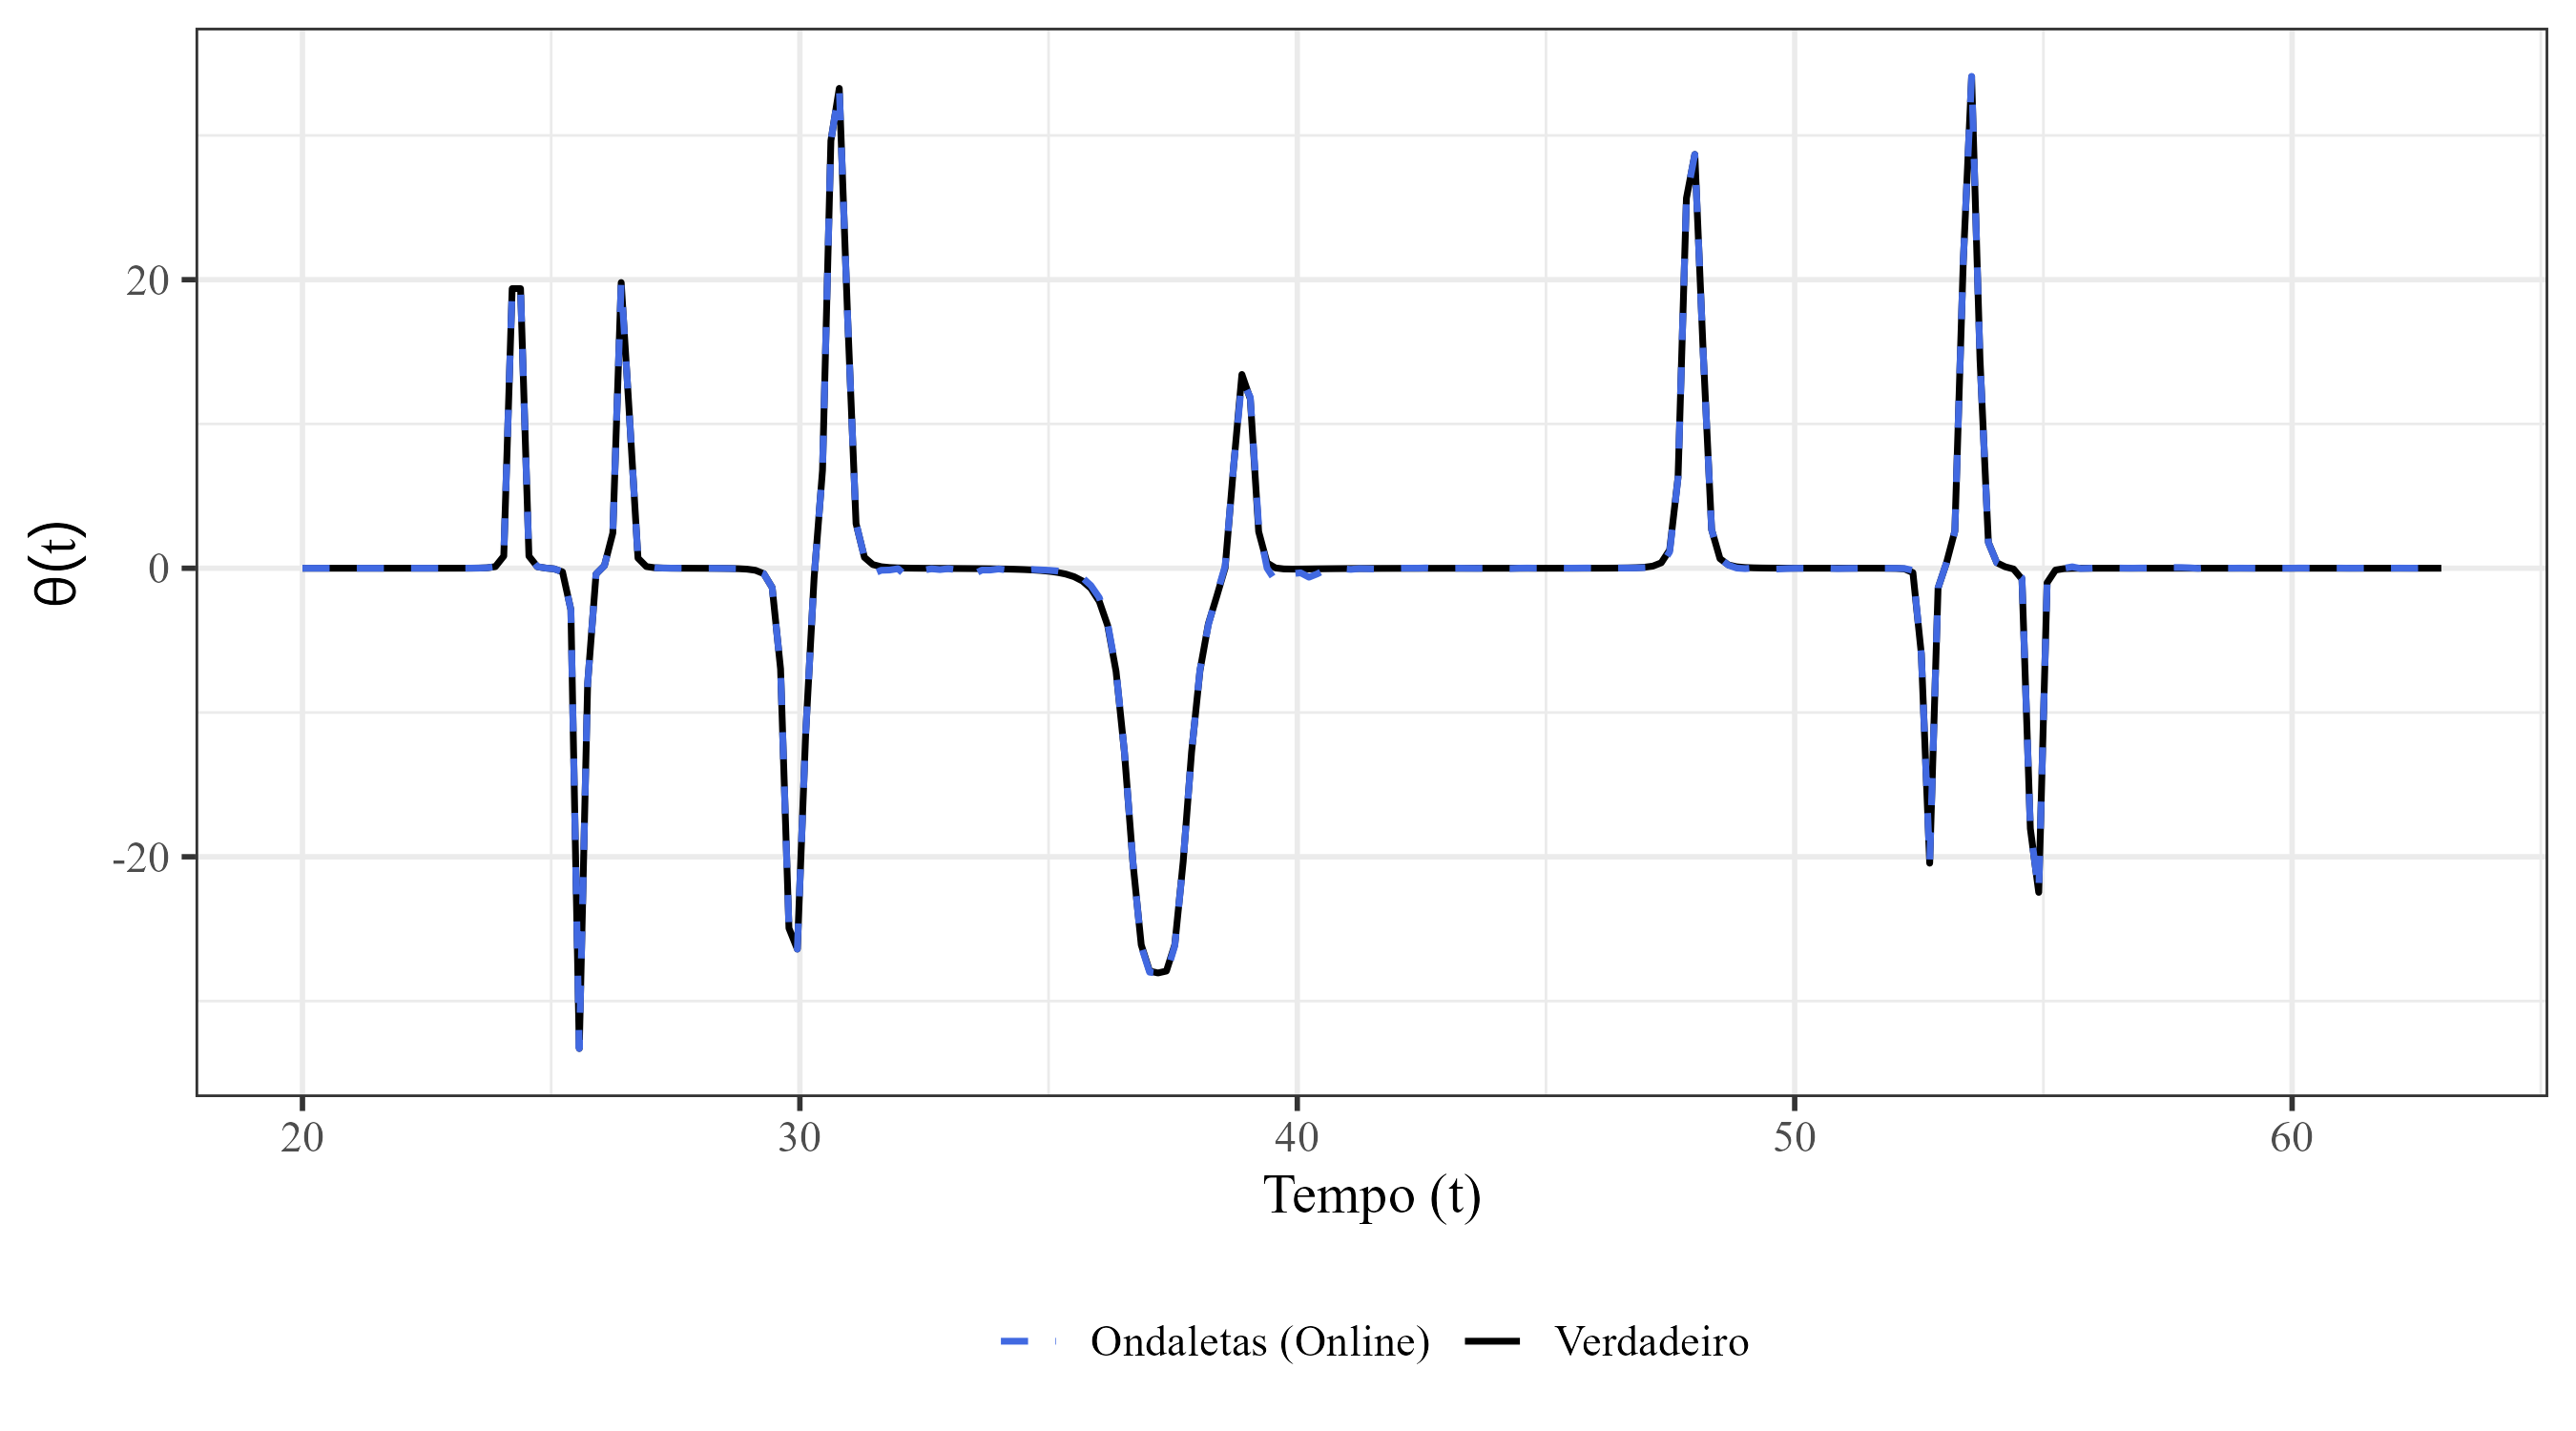
\includegraphics[height=0.95\textheight]{../figuras/sim2/texto_principal/fate_curves_Bumps.png}
\caption{\scriptsize Rastreamento \textit{online} — Bumps \((N=2000, T=512)\).}
\end{figure}
\end{frame}

\begin{frame}{Simulação 2 — Doppler}
\begin{figure}
\centering
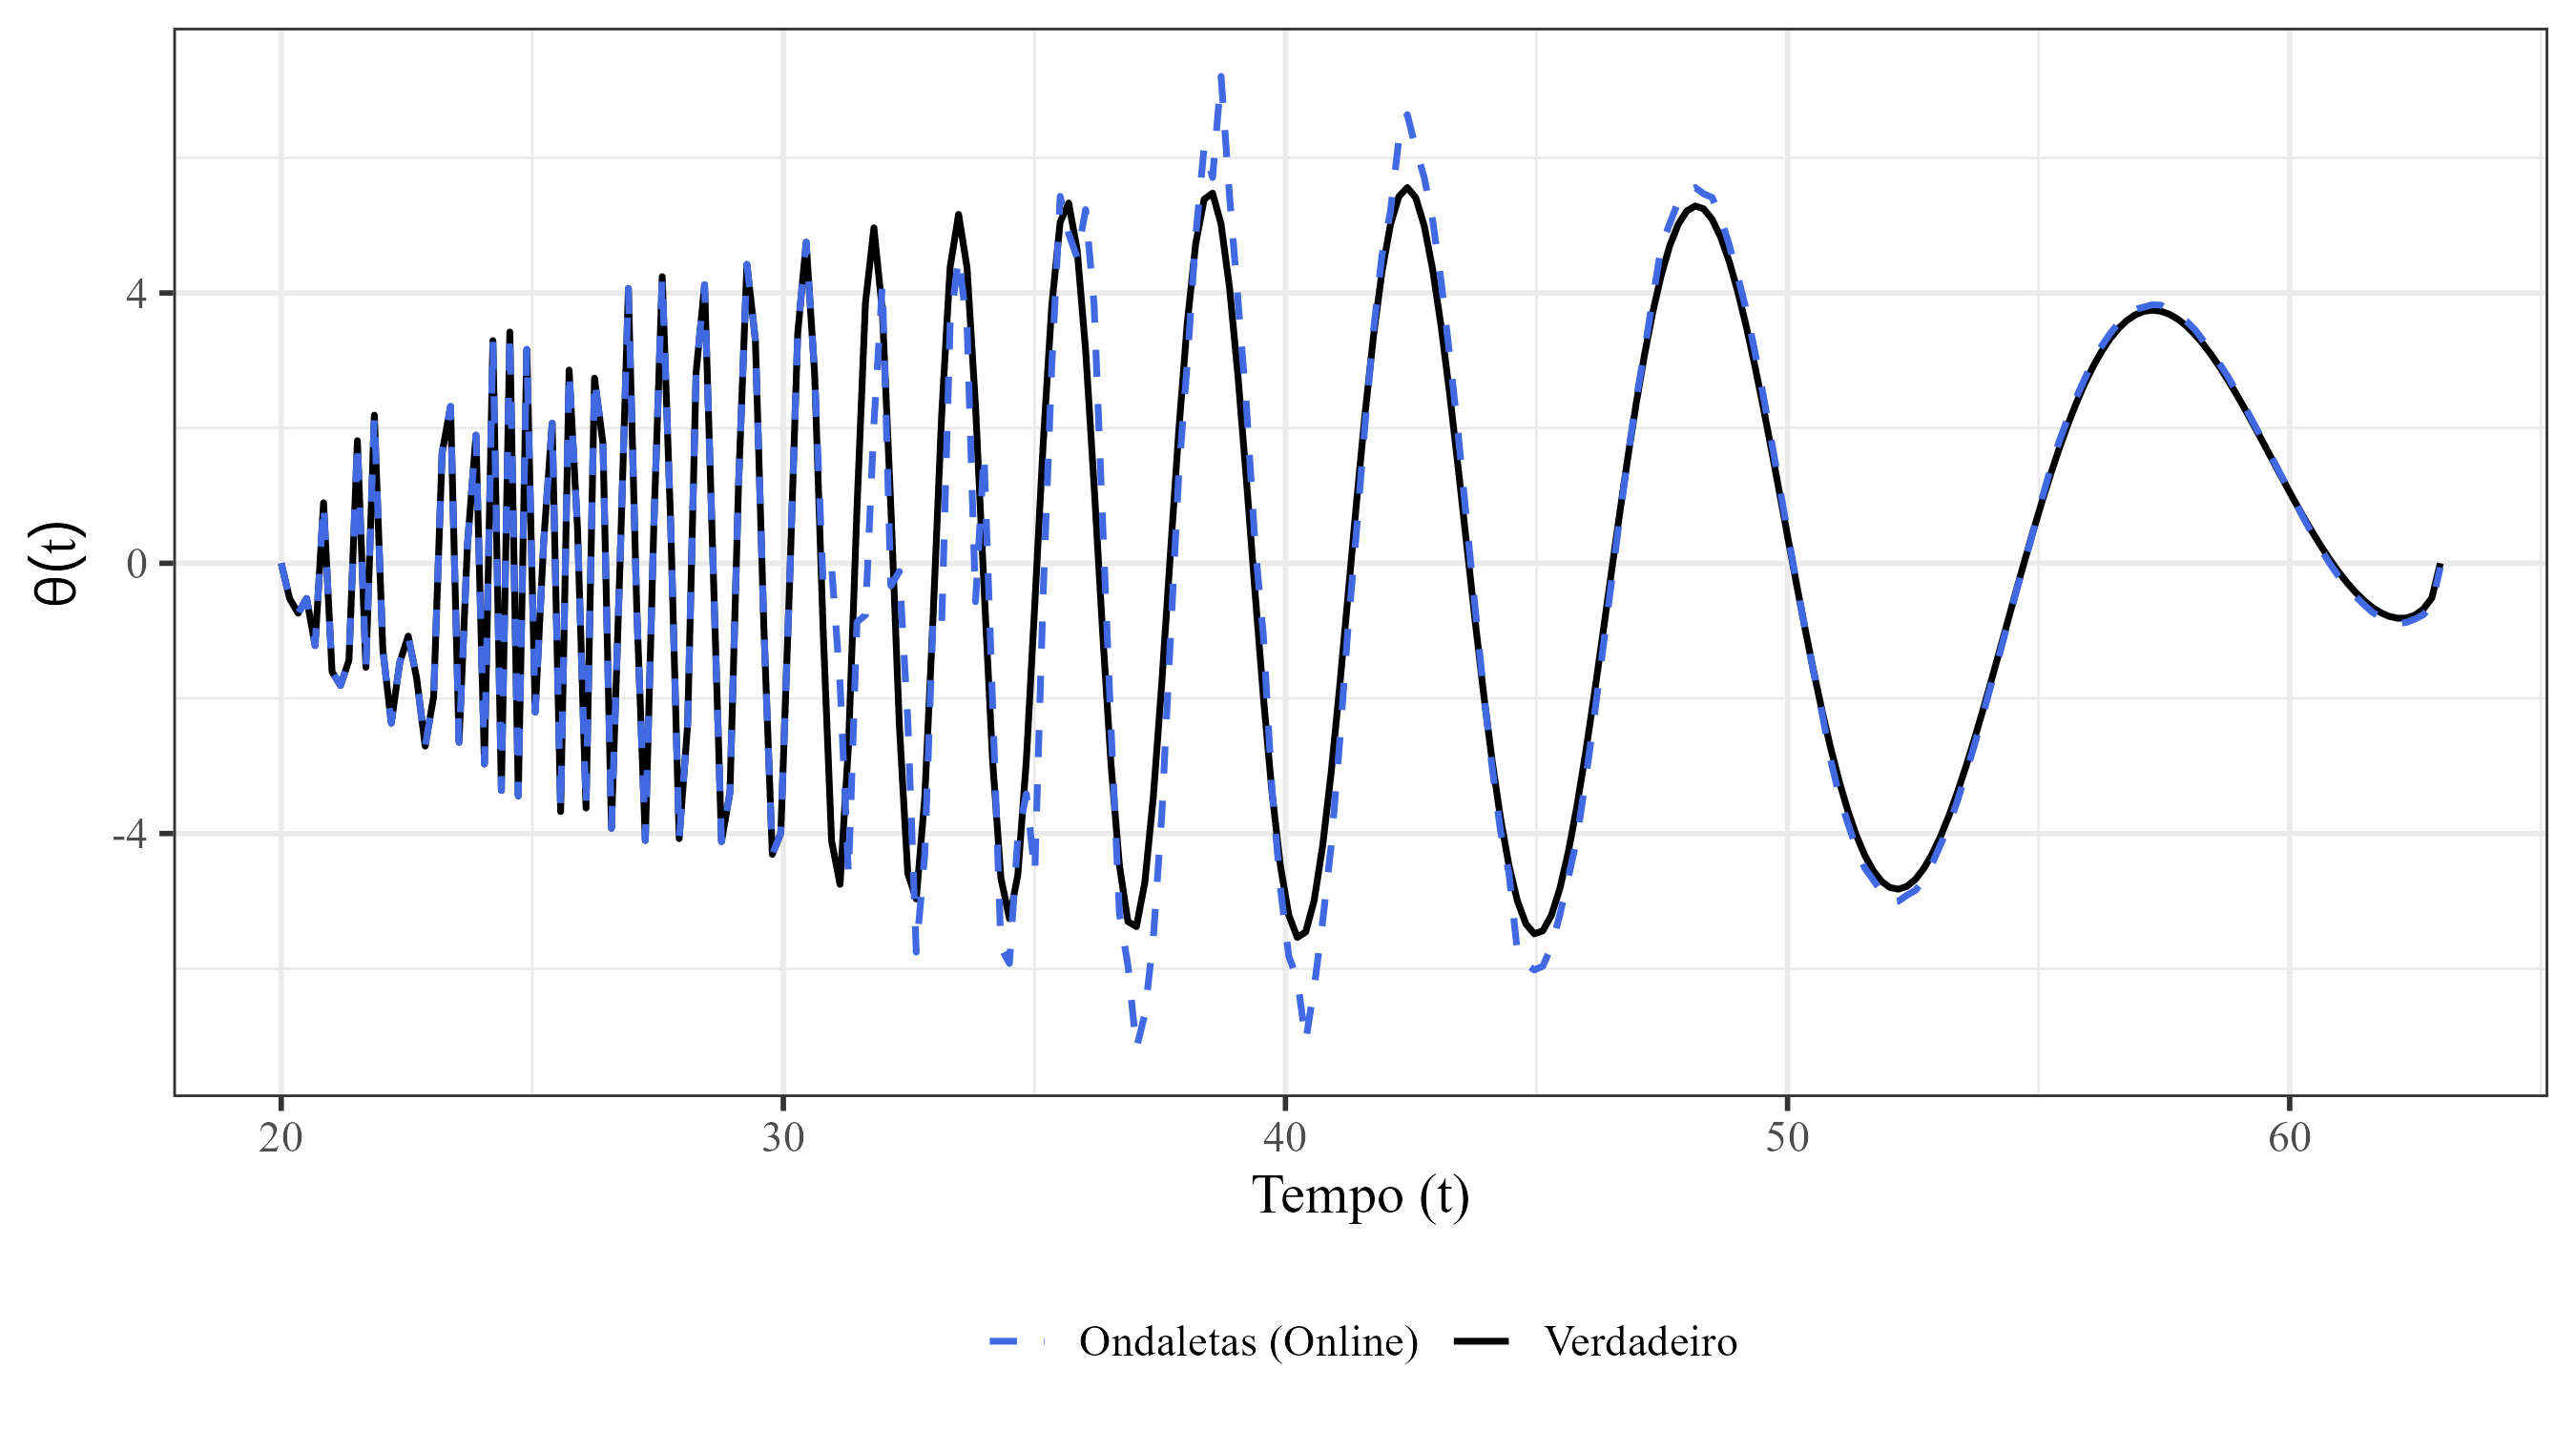
\includegraphics[height=0.72\textheight]{../figuras/sim2/texto_principal/fate_curves_Doppler.png}
\caption{\scriptsize Rastreamento \textit{online} — Doppler \((N=2000, T=512)\).}
\end{figure}
\end{frame}

% ===================================================
\section{Conclusão}
% ===================================================

\begin{frame}{Contribuições}
\begin{itemize}
    \item Estimador \textit{offline}: ondaletas via \textit{lifting} como pré-processamento do FATE; dispensa suavidade do efeito; bandas via \textit{bootstrap} não paramétrico.
    \item Estimador \textit{online}: primeira proposta sequencial do FATE com causalidade operacional; latência em microssegundos; desempenho consistente com o \textit{offline}.
    \item \texttt{rLifting}: pacote R/C++ para DWT causal; ${\approx}27\times$ mais rápido que o \texttt{wavethresh}; processamento em lote e em tempo real; extensível.
\end{itemize}
\end{frame}

\begin{frame}{Limitações}
\begin{itemize}
    \item \texttt{rLifting}: requer \(\Delta_t\) fixo; falhas de amostragem exigem interpolação prévia. Filtragem univariada: não incorpora covariância entre desfecho e confundidores. Extensão de bordas simétrica; artefatos na borda direita no modo \textit{online}.
    \item Estimador: suposições de Neyman--Rubin necessárias e difíceis de garantir; metodologia não aplicada a dados reais. Linearidade funcional assumida. Bandas \textit{bootstrap} inviáveis em tempo real estrito. Viés de limiarização presente em amostras finitas.
\end{itemize}
\end{frame}

\begin{frame}{Direções Futuras}
\begin{itemize}
    \item \texttt{rLifting} multivariado: incorporar estrutura de covariância entre desfecho e confundidores.
    \item Preditores lineares locais nas bordas: ganho direto em precisão com baixo impacto na latência.
    \item Dupla robustez: incluir modelo para a propensão \cite{testa_doubly-robust_2025}.
    \item Relaxar linearidade funcional: aprendizado de máquina funcional.
    \item Tratamentos dinâmicos e covariáveis variantes no tempo \cite{ying_causality_2024}.
\end{itemize}
\end{frame}

\begin{frame}{}
\centering
\vspace{1cm}
{\Huge \textcolor{vermelhoquaserosa}{Obrigado!}}

\vspace{1.2cm}
\large Moisés Augusto Farias da Silva

\vspace{0.3cm}
\normalsize \texttt{moisesdff8@gmail.com}

\vspace{0.8cm}
\normalsize
\textit{Orientador:} Prof.\ Dr.\ Alex Rodrigo dos Santos Sousa\\[0.2cm]
IMECC -- UNICAMP, 2026
\end{frame}

% ===================================================
\begin{frame}[allowframebreaks]{Referências}
\tiny
\bibliography{../referencias}
\end{frame}

\end{document}
